\documentclass{article}
\usepackage{tikz}
\usetikzlibrary{calc}
\usetikzlibrary{shapes.geometric, arrows.meta, positioning, decorations.markings}

\begin{document}

\begin{figure}[htbp]
\centering
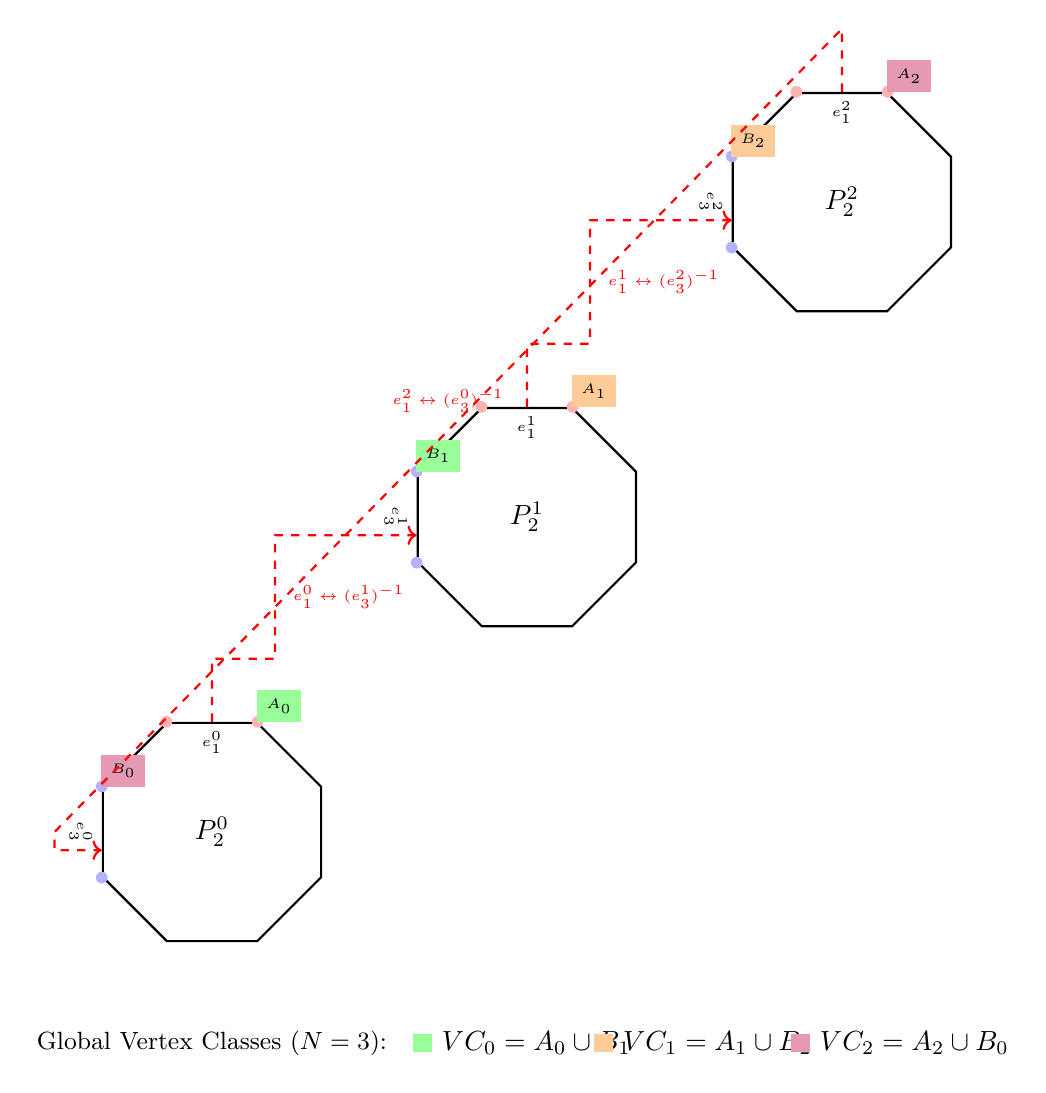
\begin{tikzpicture}[
    scale=0.8,
    octagon/.style={regular polygon, regular polygon sides=8, minimum size=3cm, draw, thick, label distance=-5mm},
    edge_label/.style={sloped, midway, font=\tiny},
    vertex_class_A/.style={fill=red!30, circle, inner sep=1.5pt},
    vertex_class_B/.style={fill=blue!30, circle, inner sep=1.5pt},
    global_vertex_1/.style={fill=green!40, font=\tiny, text=black},
    global_vertex_2/.style={fill=orange!40, font=\tiny, text=black},
    global_vertex_3/.style={fill=purple!40, font=\tiny, text=black}
]

% Define octagons
\node[octagon, label=center:$P_2^0$] (O0) at (0,0) {};
\node[octagon, label=center:$P_2^1$] (O1) at (5,5) {}; % Arranged linearly for simplicity, can be cyclic
\node[octagon, label=center:$P_2^2$] (O2) at (10,10) {};

% --- Helper to mark vertices (conceptual) ---
% Octagon 0 vertices (conceptual locations for G0A, G0B)
% G0A involves v1,v2,v5,v6,v7,v8. G0B involves v3,v4.
% Let's represent G0A near (O0.corner 1) and (O0.corner 2)
% and G0B near (O0.corner 3) and (O0.corner 4)
\node[vertex_class_A, label={[global_vertex_1, label distance=-1mm]above right:$A_0$}] at (O0.corner 1) {};
\node[vertex_class_A] at (O0.corner 2) {};
\node[vertex_class_B, label={[global_vertex_3, label distance=-1mm]above right:$B_0$}] at (O0.corner 3) {}; % B0 will connect to A2
\node[vertex_class_B] at (O0.corner 4) {};


% Octagon 1 vertices
\node[vertex_class_A, label={[global_vertex_2, label distance=-1mm]above right:$A_1$}] at (O1.corner 1) {};
\node[vertex_class_A] at (O1.corner 2) {};
\node[vertex_class_B, label={[global_vertex_1, label distance=-1mm]above right:$B_1$}] at (O1.corner 3) {}; % B1 will connect to A0
\node[vertex_class_B] at (O1.corner 4) {};

% Octagon 2 vertices
\node[vertex_class_A, label={[global_vertex_3, label distance=-1mm]above right:$A_2$}] at (O2.corner 1) {};
\node[vertex_class_A] at (O2.corner 2) {};
\node[vertex_class_B, label={[global_vertex_2, label distance=-1mm]above right:$B_2$}] at (O2.corner 3) {}; % B2 will connect to A1
\node[vertex_class_B] at (O2.corner 4) {};

% --- Labeling edges e1 and e3 (conceptual) ---
% For O0: e1 is between corner 1 and 2. e3 is between corner 3 and 4.
\path (O0.corner 1) -- (O0.corner 2) node[edge_label, midway, below] {$e_1^0$};
\path (O0.corner 3) -- (O0.corner 4) node[edge_label, midway, below] {$e_3^0$};

% For O1:
\path (O1.corner 1) -- (O1.corner 2) node[edge_label, midway, below] {$e_1^1$};
\path (O1.corner 3) -- (O1.corner 4) node[edge_label, midway, below] {$e_3^1$};

% For O2:
\path (O2.corner 1) -- (O2.corner 2) node[edge_label, midway, below] {$e_1^2$};
\path (O2.corner 3) -- (O2.corner 4) node[edge_label, midway, below] {$e_3^2$};

% --- Indicating connections (conceptual) ---
% Based on the provided image image_51cb18.png
% Assumes O0, O1, O2 nodes (octagons) are already defined and positioned.

% Define coordinates for edge connection points for clarity
% Using 0.5 for starting edges (e.g., e1^j) and user's 0.7 for target edges (e.g., e3^k)
\coordinate (e1O0start)  at ($(O0.corner 1)!0.5!(O0.corner 2)$);
\coordinate (e3O1target) at ($(O1.corner 3)!0.7!(O1.corner 4)$); % Target on e3_1 of O1

\coordinate (e1O1start)  at ($(O1.corner 1)!0.5!(O1.corner 2)$);
\coordinate (e3O2target) at ($(O2.corner 3)!0.7!(O2.corner 4)$); % Target on e3_2 of O2

\coordinate (e1O2start)  at ($(O2.corner 1)!0.5!(O2.corner 2)$); % Starting from e1_2 on O2
\coordinate (e3O0target) at ($(O0.corner 3)!0.7!(O0.corner 4)$); % Target on e3_0 of O0

% Connection 1: e1^0 (on O0) paired with (e3^1)^-1 (on O1)
% Path style from image: Horizontal right, then Vertical up, then Horizontal right to target.
% Arrow O0 -> O1
\draw[->, thick, red, dashed]
  (e1O0start) % Start from midpoint of e1_0 on O0
  -- ++(0.0,1.0)
  -- ++(1.0,0) coordinate (P0_HsegEnd) % 1. Horizontal segment to the right (adjust 1.0 as needed)
  -- (P0_HsegEnd |- e3O1target) % 2. Vertical segment up/down to the Y-level of the target point on e3_1
  node[pos=0.5, right, font=\tiny, xshift=1mm] {$e_1^0 \leftrightarrow (e_3^1)^{-1}$} % Label on the vertical segment
  -- (e3O1target); % 3. Horizontal segment to the target point on e3_1

% Connection 2: e1^1 (on O1) paired with (e3^2)^-1 (on O2)
% Path style from image: Similar H-V-H structure.
% Arrow O1 -> O2
\draw[->, thick, red, dashed]
  (e1O1start) % Start from midpoint of e1_1 on O1
  -- ++(0.0,1.0)
  -- ++(1.0,0) coordinate (P1_HsegEnd) % 1. Horizontal segment to the right (adjust 1.0)
  -- (P1_HsegEnd |- e3O2target) % 2. Vertical segment up/down to the Y-level of the target point on e3_2
  node[pos=0.5, right, font=\tiny, xshift=1mm] {$e_1^1 \leftrightarrow (e_3^2)^{-1}$} % Label on the vertical segment
  -- (e3O2target); % 3. Horizontal segment to the target point on e3_2

% Connection 3: e1^2 (on O2) paired with (e3^0)^-1 (on O0) - CYCLIC
% Path style from image: Vertical up from O2, then long Horizontal left, then Vertical down, then Horizontal to target on O0.
% Arrow O2 -> O0 (following the image's direction for this specific connection)
\draw[->, thick, red, dashed]
  (e1O2start) % Start from midpoint of e1_2 on O2
  -- ++(0,1.0) coordinate (P2_VsegEnd) % 1. Vertical segment up (adjust 1.5)
  -- ($(O0) + (-2.5,0)$ |- P2_VsegEnd) coordinate (P2_HsegEnd) % 2. Long horizontal segment to the left
                                                             % (X is 2.5 units left of O0's center, Y is P2_VsegEnd's Y)
  node[pos=0.5, above, font=\tiny, yshift=1mm] {$e_1^2 \leftrightarrow (e_3^0)^{-1}$} % Label on this long horizontal segment
  -- (P2_HsegEnd |- e3O0target) % 3. Vertical segment down to the Y-level of the target on e3_0
  -- (e3O0target); % 4. Horizontal segment to the target point on e3_0 (this segment might be short)

% --- Global Vertex Classes (Conceptual Legend) ---
\node[below=1cm of O0, font=\small] (legend_title) {Global Vertex Classes ($N=3$):};
\node[global_vertex_1, right=0.2cm of legend_title, label=right:{$VC_0 = A_0 \cup B_1$}] {};
\node[global_vertex_2, right=2.5cm of legend_title, label=right:{$VC_1 = A_1 \cup B_2$}] {};
\node[global_vertex_3, right=5cm of legend_title, label=right:{$VC_2 = A_2 \cup B_0$}] {};

\end{tikzpicture}

\caption{Schematic illustration of $N=3$ octagons forming a $Z_3$-symmetric chain.
Red dashed arrows indicate the primary gluing $e_1^j \leftrightarrow (e_3^{(j+1)})^{-1}$ which cyclically connects the octagons.
Colored circles conceptually mark the local vertex classes ($A_j$ in red, $B_j$ in blue) and their grouping into $N=3$ distinct global vertex classes ($VC_0, VC_1, VC_2$ shown with distinct label background colors like green, orange, purple).
Each global vertex class arises from identifying an $A$-type class from one octagon with a $B$-type class from the next, demonstrating how $N$ distinct vertices are formed in $S_g$.
The $8N$ original vertices fall into $N$ orbits under $\Gamma_g$.}

\end{figure}

\end{document}